\documentclass[AMS,STIX2COL]{WileyNJD-v2}

\articletype{Article Type}
\received{26 April 2016}
\revised{6 June 2016}
\accepted{6 June 2016}
\raggedbottom

\begin{document}
    \title{Improvement of Korean Morphological Analysis System \\Through Transformer-Based Re-Ranking}

    \author[1]{Author One*}
    \author[2,3]{Author Two}
    \author[3]{Author Three}
    \authormark{AUTHOR ONE \textsc{et al}}

    \address[1]{\orgdiv{Org Division}, \orgname{Org Name}, \orgaddress{\state{State name}, \country{Country name}}}
    \address[2]{\orgdiv{Org Division}, \orgname{Org Name}, \orgaddress{\state{State name}, \country{Country name}}}
    \address[3]{\orgdiv{Org Division}, \orgname{Org Name}, \orgaddress{\state{State name}, \country{Country name}}}
    \corres{*Corresponding author name, This is sample corresponding address. \email{authorone@gmail.com}}
    \presentaddress{This is sample for present address text this is sample for present address text}

    \abstract[Abstract]{
        Korean morphological analysis is a fundamental step in analyzing the Korean language.
        Owing to the nature of Korean agglutinative words, building an automatic analysis system is difficult because parts-of-speech tagging independently is insufficient to complete analysis, as in English.
        In addition, various methods for morphological analysis have been proposed; however, efficient methods, such as BPE (Byte Pair Encoding), are mainly used in applications intended to be used as tokenizers for deep learning.
        In this study, we propose a method to maximize the performance of an efficient morphological analysis system that can be used for tokenization through multi-stage re-ranking based on deep learning.
        For cases whose rankings have been changed through re-ranking, it is feasible to improve the performance while maintaining speed by updating the cost matrix of the lattice-based morphological analysis system.
        Through experiments, we demonstrate that the proposed method effectively improves performance via reducing errors by over 30\% in both spoken and written language models.
    }
    \keywords{Korean morphological analysis, natural language understanding, deep learning, pretrained transformer encoder, re-ranking}

    \JELinfo{classification}
    \MSC{Code numbers}
    \jnlcitation{\cname{
        \author{Williams K.},
        \author{B. Hoskins},
        \author{R. Lee},
        \author{G. Masato}, and \author{T. Woollings}} (\cyear{2016}),
        \ctitle{A regime analysis of Atlantic winter jet variability applied to evaluate HadGEM3-GC2}, \cjournal{Q.J.R. Meteorol. Soc.}, \cvol{2017;00:1--6}.}
    \maketitle
    \footnotetext{\textbf{Abbreviations:} ANA, anti-nuclear antibodies; APC, antigen-presenting cells; IRF, interferon regulatory factor}


    \begin{center}
        \begin{table*}[t]
            \caption{Maximum performance of alternative paths as correct answers}\label{tab:maximum-performance}
            \centering
            \begin{tabular*}{500pt}{@{\extracolsep\fill}cccD{.}{.}{3}c@{\extracolsep\fill}}
                \toprule
                & \multicolumn{2}{@{}c@{}}{\textbf{Written Language Evaluation Set}} & \multicolumn{2}{@{}c@{}}{\textbf{Spoken Language Evaluation Set}} \\\cmidrule{2-3}\cmidrule{4-5}
                alternative range & eojeol accuracy & average number of alternative & \multicolumn{1}{@{}l@{}}{eojeol accuracy}  & average number of alternative \\
                \midrule
                no alternative    & 96.36           & 1.0                           & 92.54                                     & 1.0                           \\
                secondary         & 98.74           & 25.7                          & 97.27                                     & 12.9                          \\
                tertiary          & 98.96           & 47.8                          & 97.81                                     & 23.6                          \\
                quarternary       & 99.01           & 69.6                          & 97.95                                     & 34.2                          \\
                quinary           & 99.02           & 91.1                          & 98.01                                     & 44.5                          \\
                \bottomrule
            \end{tabular*}
            \begin{tablenotes}
                \footnotesize
                \item\hspace{2mm} * Written Language Evaluation Set: 2,400 sentences each randomized from UCorpus and Everyone Corpus (4,800 sentences total)
                \item\hspace{2mm} * Spoken Language Evaluation Set: 2,400 sentences each randomized from UCorpus and Everyone Corpus (4,800 sentences total)
            \end{tablenotes}
        \end{table*}
    \end{center}


    \section{Introduction}\label{sec:intro}

    Korean morphological analysis is the process of determining parts of speech by identifying morphemes, which are the smallest units of linguistic expression with independent meanings in a sentence.
    In an isolating language, such as English, this identification can be achieved relatively easily by tagging parts of speech sequentially.
    However, in Korean, the nature of the agglutinative language requires separating endings or postpositions and restoring inflections to their original form.
    In addition, because the basic input of other Korean analysis tasks is often a separate morpheme, the accuracy of the morphological analysis significantly affects the performance of Korean analysis.
    Modern high-performance deep learning methods in natural language processing (NLP) use a tokenization process that breaks the text into smaller units and converts each token into a vector as an input to the computational model~\cite{Mikolov2013}.
    Here, the token unit is mainly a subword unit, and to reflect the characteristics of a Korean subword, tokenization with separate morphemes is attempted in advance~\cite{SongHJ2021}.
    Using the results of the morphological analysis for this tokenization process improves the overall performance of the analysis by reflecting the semantic units of Korean.
    This requires a highly accurate and fast morphological analyzer.

    Various approaches have been proposed for morphological analysis, which is crucial in Korean language analysis~\cite{KwonHC1991, LeeDG2009, ShimKS2011, LeeJS2011, ShinJC2012, LeeCK2013, NaSH2014, NaSH2015, HwangHS2016, KimHM2016, ChungES2016, LeeCH2016, Li2017, NaSH2018, KimSW2018, ChoiYS2018, MinJW2018, MinJW2019, KimHM2019, SongHJ2019, MinJW2020, SongHJ2020, ChoiYS2020, HwangHS2020, KimHJ2021, YounJY2021, MinJW2022, KimJM2022, ShinHJ2023}.
    In general, when people understand speech or written text, they attempt to make sense of it using vocabulary and concepts that they are familiar with.
    While there are approaches to use rules or dictionaries to reflect this understanding~\cite{KwonHC1991}, it becomes difficult to build and maintain a dictionary for the vocabulary that appears in each text.
    Therefore, methods for tagging syllable units without a dictionary have been proposed~\cite{ShimKS2011, LeeCK2013, LeeCH2016, KimHM2016} and studies have been conducted to improve them ~\cite{KimSW2018, ChoiYS2018, KimHM2019, MinJW2019, SongHJ2019, SongHJ2020, YounJY2021, ShinHJ2023}.
    From a mechanical perspective, syllable-by-syllable morphological analysis can be performed either by tagging syllable-by-syllable and then applying a base-form restoration dictionary~\cite{ShimKS2011, LeeCH2016}, or by tagging syllable-by-syllable with the base form already restored~\cite{YounJY2021}.
    However, syllable-by-syllable morphological analysis has limitations, in that it is difficult to accurately identify morpheme boundaries and learn long-term contextual information as the length of the sequence increases.
    In this study, the former is referred to as dictionary-based morphological analysis and the latter as syllable-unit morphological analysis.
    Both methods are trained on a manually labeled corpus and cannot accurately analyze new syllable combinations or morphemes that do not appear in the training corpus.
    Recently, with the development of the Internet and the spread of open sources as well as open data, web texts, corpora, language resources, and knowledge shared by different people have accumulated significantly.
    The reduced cost of building and maintaining a dictionary provides a significant opportunity to overcome the limitations of dictionary-based methods.

    Against this background, this study considers how the dictionary-based morphological analysis method used by MeCab~\cite{MeCab}, an open software for Korean and Japanese morphological analysis in tokenizers, which is an essential preprocessing tool for deep learning, can be effectively improved, and a method is proposed.
    The dictionary-based morphological analysis method~\cite{Kudo2004, NaSH2014, NaSH2015, NaSH2018} trained by the CRF (Conditional Random Fields) method~\cite{Lafferty2001} lists the candidate morphemes in the dictionary from a given sentence to form a lattice structure connected by a directed graph and determines the optimal morphological analysis path within it.
    The process of determining the optimal path in the lattice uses the Viterbi algorithm~\cite{Viterbi1967}, which determines the path that minimizes the cost of each morpheme node and the sum of the neighborhood costs of two consecutive morphemes.
    The main types of errors in these dictionary-based morphological analysis methods occur when new words that are not in the dictionary are used in a sentence, or when the optimal path calculation selects the incorrect result owing to bias.
    For example, it may be cost-effective to select one long morpheme than several short morphemes, but this may often lead to an incorrect analysis.
    The main motivation for this study was that the path that minimizes the costs for the nodes and links may not be the optimal path.

    To identify cases in which a suboptimal solution is actually the best solution according to the best path calculation, we modified the best path calculation method to generate suboptimal analysis results and verified the extent to which they are correct.
    Although there are numerous different approaches to select the next-best path, we used the method of replacing a morpheme node on the optimal path with a lower-ranked node.
    As shown in Table~\ref{tab:maximum-performance}, we confirm the extent to which the analysis performance can be improved by replacing the optimal path with a lower-ranked node.
    We can consider the problem of finding the correct answer among the generated sub-optimals, similar to the problem of re-ranking search results in information retrieval~\cite{BaeYJ2021}.
    In ~\cite{ChoiYS2018}, the N-best analysis results generated by the seq2seq model were re-ranked based on a convolutional neural network to improve the performance.
    In this study, re-ranking was performed using two BERT models of different types and forms, as proposed in ~\cite{Nogueira2019}.
    Experimental results show that first-stage re-ranking improves the performance by over 20\% over previously written and spoken models, and second-stage re-ranking with a different type of input and a different type of pre-trained model further improves the performance by more than 30\% over previously written and spoken models.

    With this method, the performance of the dictionary-based morphological analysis method could be further improved; however, the overall analysis time increased when the morphological analysis system was configured, including the re-ranking model itself.
    However, it is feasible to use the results of multiple reranked morpheme analyses to update the connection costs between morphemes in a dictionary, similar to the backpropagation process in a typical neural network.
    It is also expected that the morphological analysis system with improved connection costs will be able to generate better re-ranking candidates, which will further improve performance by doing so iteratively.
    Further research is required in the future.
    In this study, only performance improvement using the second-stage re-ranking was covered as the scope of the study.
    The main contributions of this study are as follows.
    \begin{enumerate}
        \item \textbf{Further improvement of dictionary-based morphological analysis method using suboptimal analysis results}: We explore the possibility of performance improvement by introducing a method to replace the optimal path with a suboptimal node and propose a method to effectively improve the dictionary-based morphological analysis method through deep learning.
        \item \textbf{Extending the performance improvement by introducing a two-stage re-ranking model}: To improve the performance of dictionary-based analysis by re-ranking the morphological analysis results, we propose extending the performance improvement using different BERT models to perform two rounds of re-ranking.
        \item \textbf{A method for updating connection costs in the dictionary and suggestions for future research}: We propose a new method for updating dictionary connection costs based on re-ranked morphological analysis results. We also outline directions for future research, suggesting potential improvements.
    \end{enumerate}
    These contributions provide important insights into the performance improvement of Korean morphological analysis and the direction of future research, and will serve as a useful reference for future researchers.

    The remainder of this paper is organized as follows.
    In Section ~\ref{sec:related-work}, we introduce previous research cases related to this study.
    In Section ~\ref{sec:morphological-analysis-model}, we discuss configuring and training a dictionary-based morphological analysis system.
    In Section ~\ref{sec:re-ranking-model}, we discuss the generation of secondary results of morphological analysis, produce re-ranking data, and propose a method for training a two-stage re-ranking model.
    In Section ~\ref{sec:results}, we discuss the results of the performance improvement using the morphological analysis and re-ranking models.
    Finally, in Section ~\ref{sec:conclusion}, we conclude the study and discuss its limitations and directions for future research.


    \begin{figure*}[t]
        \centerline{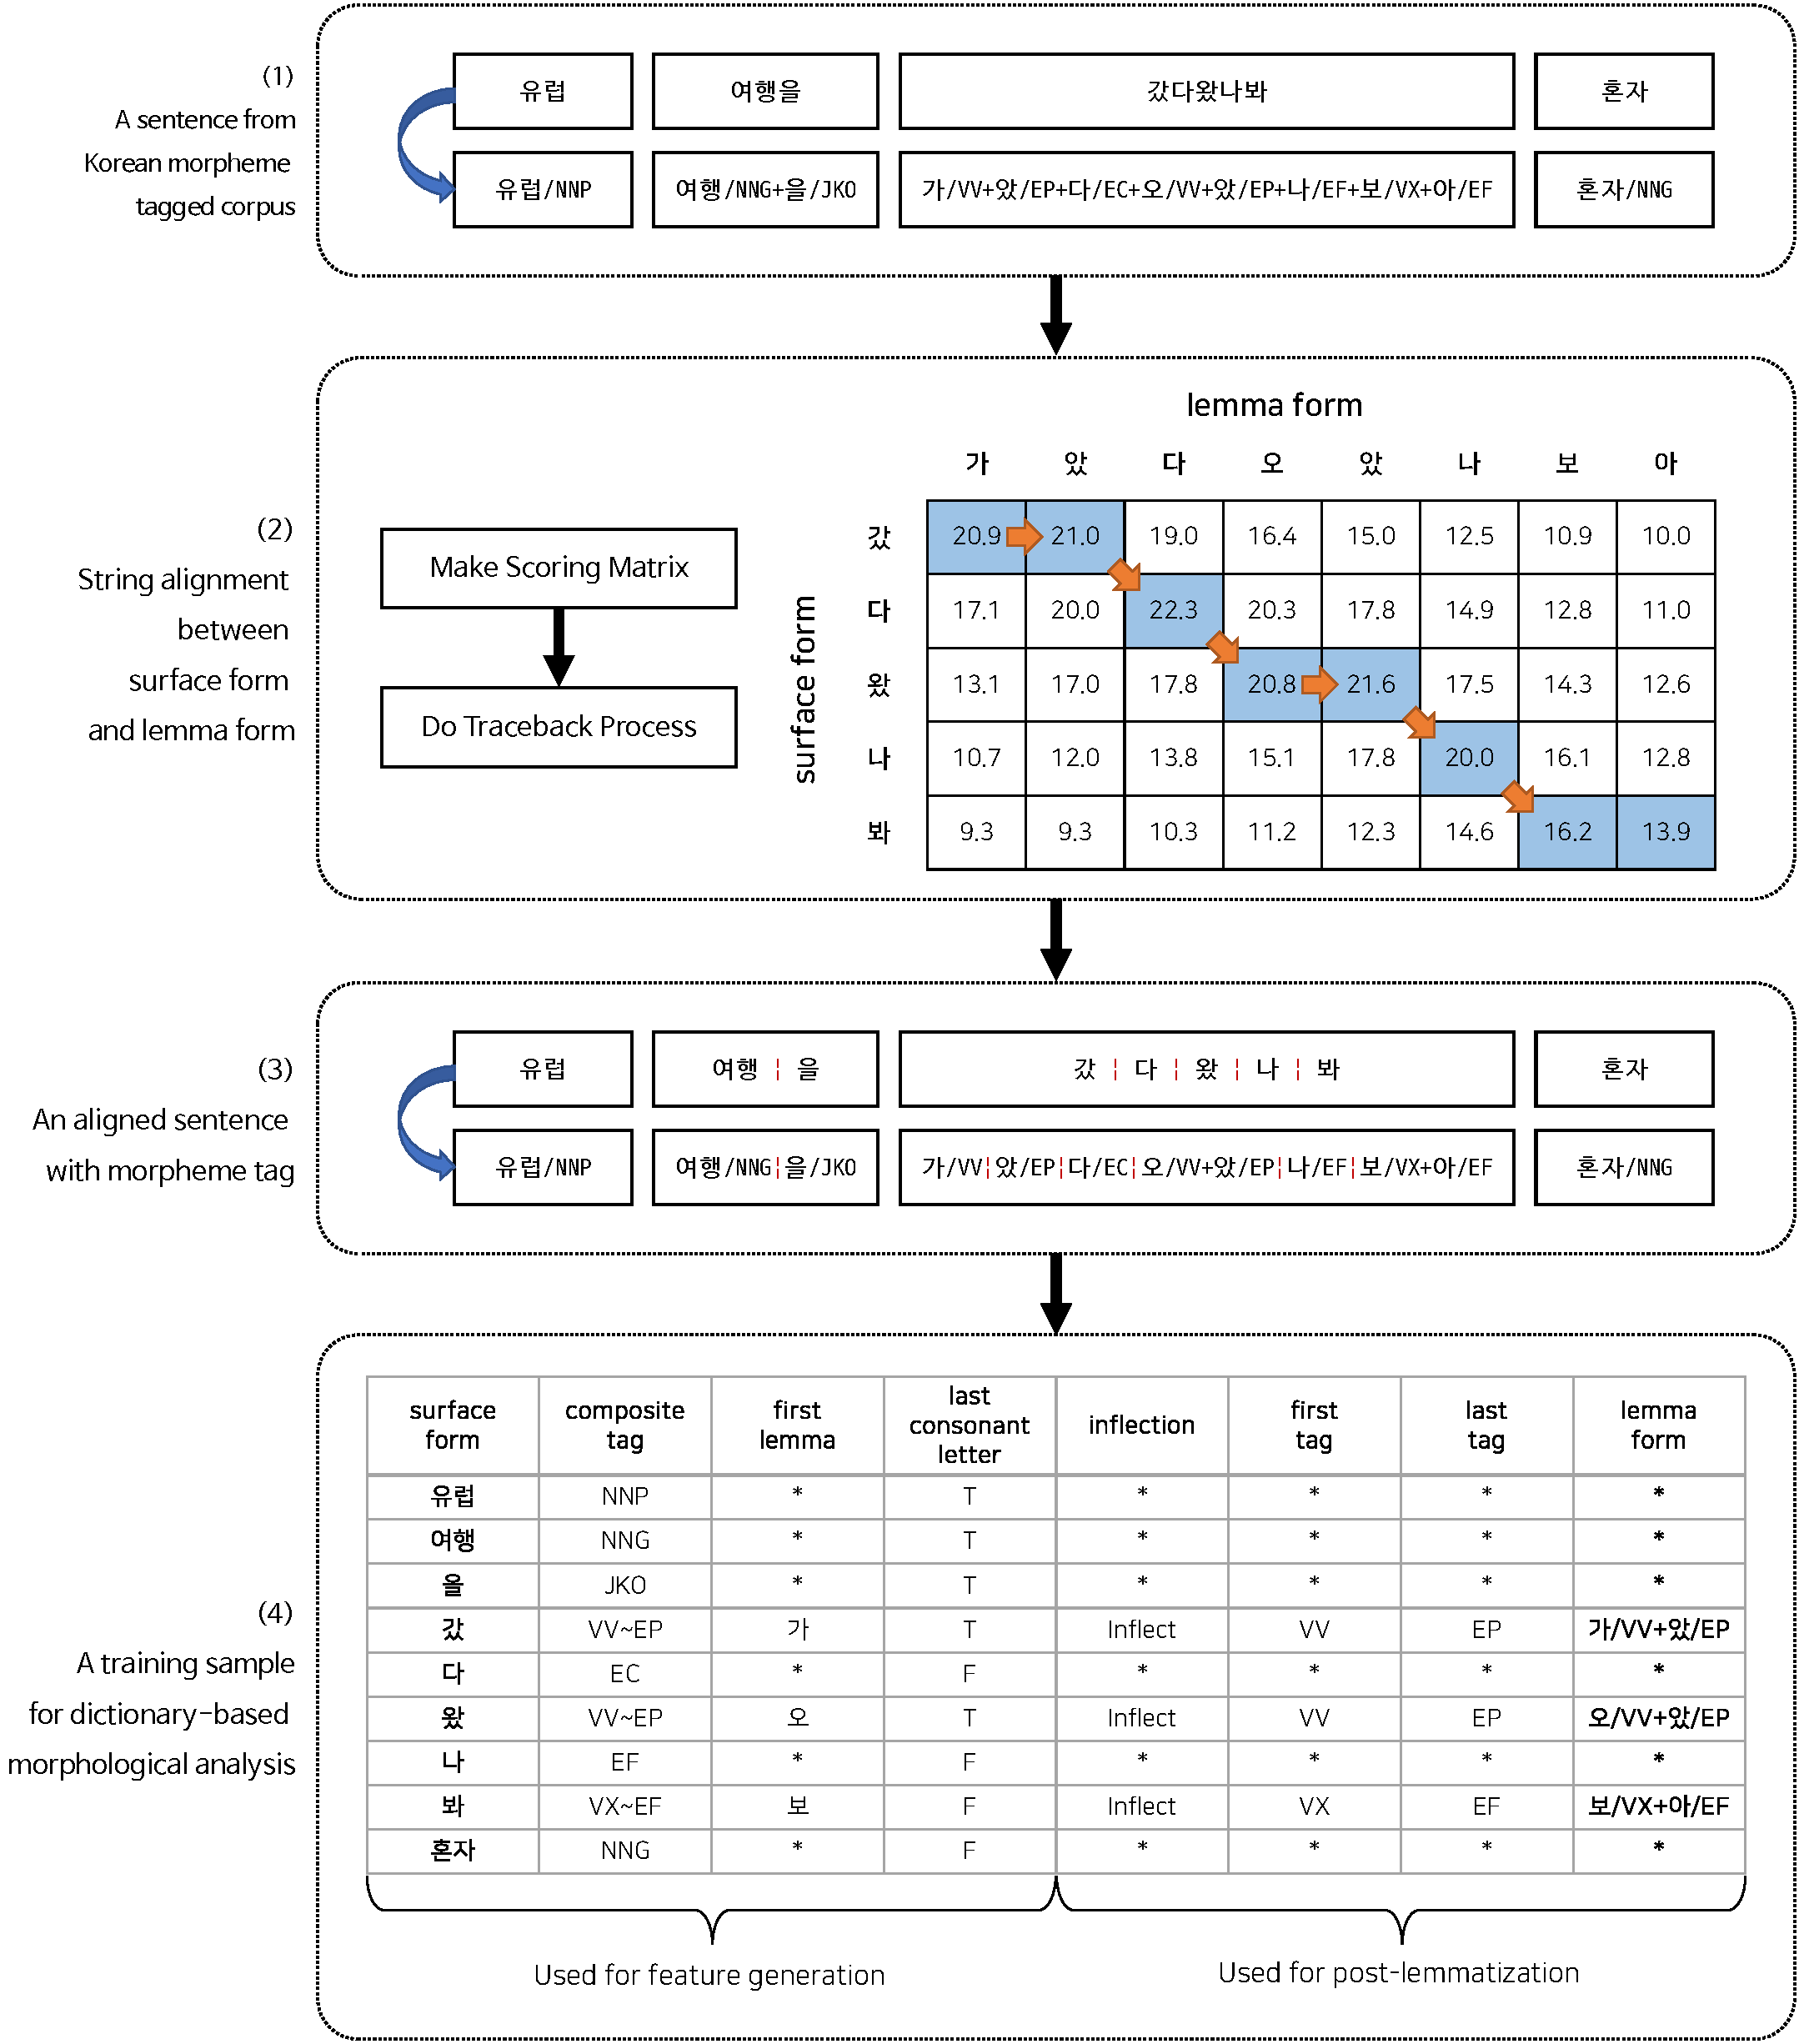
\includegraphics[width=0.75\textwidth]{fig1.1}}
        \caption{Transformation of a single sentence in the Korean morpheme-tagged corpus into a single training sample}\label{fig:sample}
    \end{figure*}


    \section{Related Work}\label{sec:related-work}

    Korean morphological analyses have seen an influx of various methodologies in recent years~\cite{KwonHC1991, LeeDG2009, ShimKS2011, LeeJS2011, ShinJC2012, LeeCK2013, NaSH2014, NaSH2015, HwangHS2016, KimHM2016, ChungES2016, LeeCH2016, Li2017, NaSH2018, KimSW2018, ChoiYS2018, MinJW2018, MinJW2019, KimHM2019, SongHJ2019, MinJW2020, SongHJ2020, ChoiYS2020, HwangHS2020, KimHJ2021, YounJY2021, MinJW2022, KimJM2022, ShinHJ2023}.
    The nature of the Korean language, being agglutinative, introduces challenges that have propelled researchers to develop inventive solutions, many of which have laid the groundwork for future research.

    \subsection{Traditional Dictionary-based Approaches}\label{subsec2.1}
    The earliest attempts at Korean morphological analysis relied heavily on rule- and dictionary-based methods~\cite{KwonHC1991}.
    These methodologies employ predefined sets of linguistic rules or large dictionaries to detect morphemes and determine parts of speech.
    One of the most significant advantages of this approach is its deterministic nature, which can lead to high accuracy when the input text closely adheres to the rules or dictionaries used.
    However, it is challenging to scale and update them, particularly with the constant evolution of language and the emergence of new words.
    The dynamic nature of language, particularly in the Internet age, has made the maintenance of comprehensive dictionaries labor-intensive.

    \subsection{Syllable-unit Morphological Analysis}\label{subsec2.2}
    To overcome the limitations of dictionary dependence, syllable-by-syllable morphological analysis has emerged as an alternative~\cite{ShimKS2011, LeeCK2013, LeeCH2016, KimHM2016, KimSW2018, ChoiYS2018, KimHM2019, MinJW2019, SongHJ2019, SongHJ2020, YounJY2021, ShinHJ2023}.
    This method either tags each syllable and then applies a base-form restoration dictionary~\cite{ShimKS2011, LeeCH2016} or tags the syllable with the base form already restored~\cite{YounJY2021}.
    One notable drawback is the challenge of accurately pinpointing morpheme boundaries.
    Furthermore, as the sequences increase in length, the system finds it increasingly challenging to understand long-term contextual data.

    \subsection{Deep Learning and Tokenization}\label{subsec2.3}
    The advent of deep learning has reshaped the Korean morphological analysis landscape.
    High-performance deep learning models in NLP employ tokenization, dividing the text into smaller units and then converting these tokens into vectors as an input to the computational model~\cite{Mikolov2013}.
    The attempt to conduct subword tokenization, incorporating separate morphemes to cater to Korean linguistic characteristics is particularly significant.
    Incorporating accurate morpheme analysis results into tokenization can improve overall analysis performance.

    With advancements in technology and access to large datasets, the potential to integrate dictionary-based methods with deep learning techniques has emerged.
    As motivated in our study, MeCab~\cite{MeCab}, an open software for Korean and Japanese morphological analysis, utilized dictionary-based morphological analysis trained by the CRF method~\cite{Lafferty2001}.
    This method attempts to find the optimal morphological analysis path by forming a lattice structure as in ~\cite{Kudo2004, NaSH2014, NaSH2015, NaSH2018}.
    The amalgamation of dictionary-based methods with deep learning, as explored in our research, signifies the latest strides in this journey aimed at harnessing the strengths of both approaches.
    Future research avenues include refining these hybrid methods and exploring the capabilities of end-to-end models.


    \begin{figure*}[t]
        \centerline{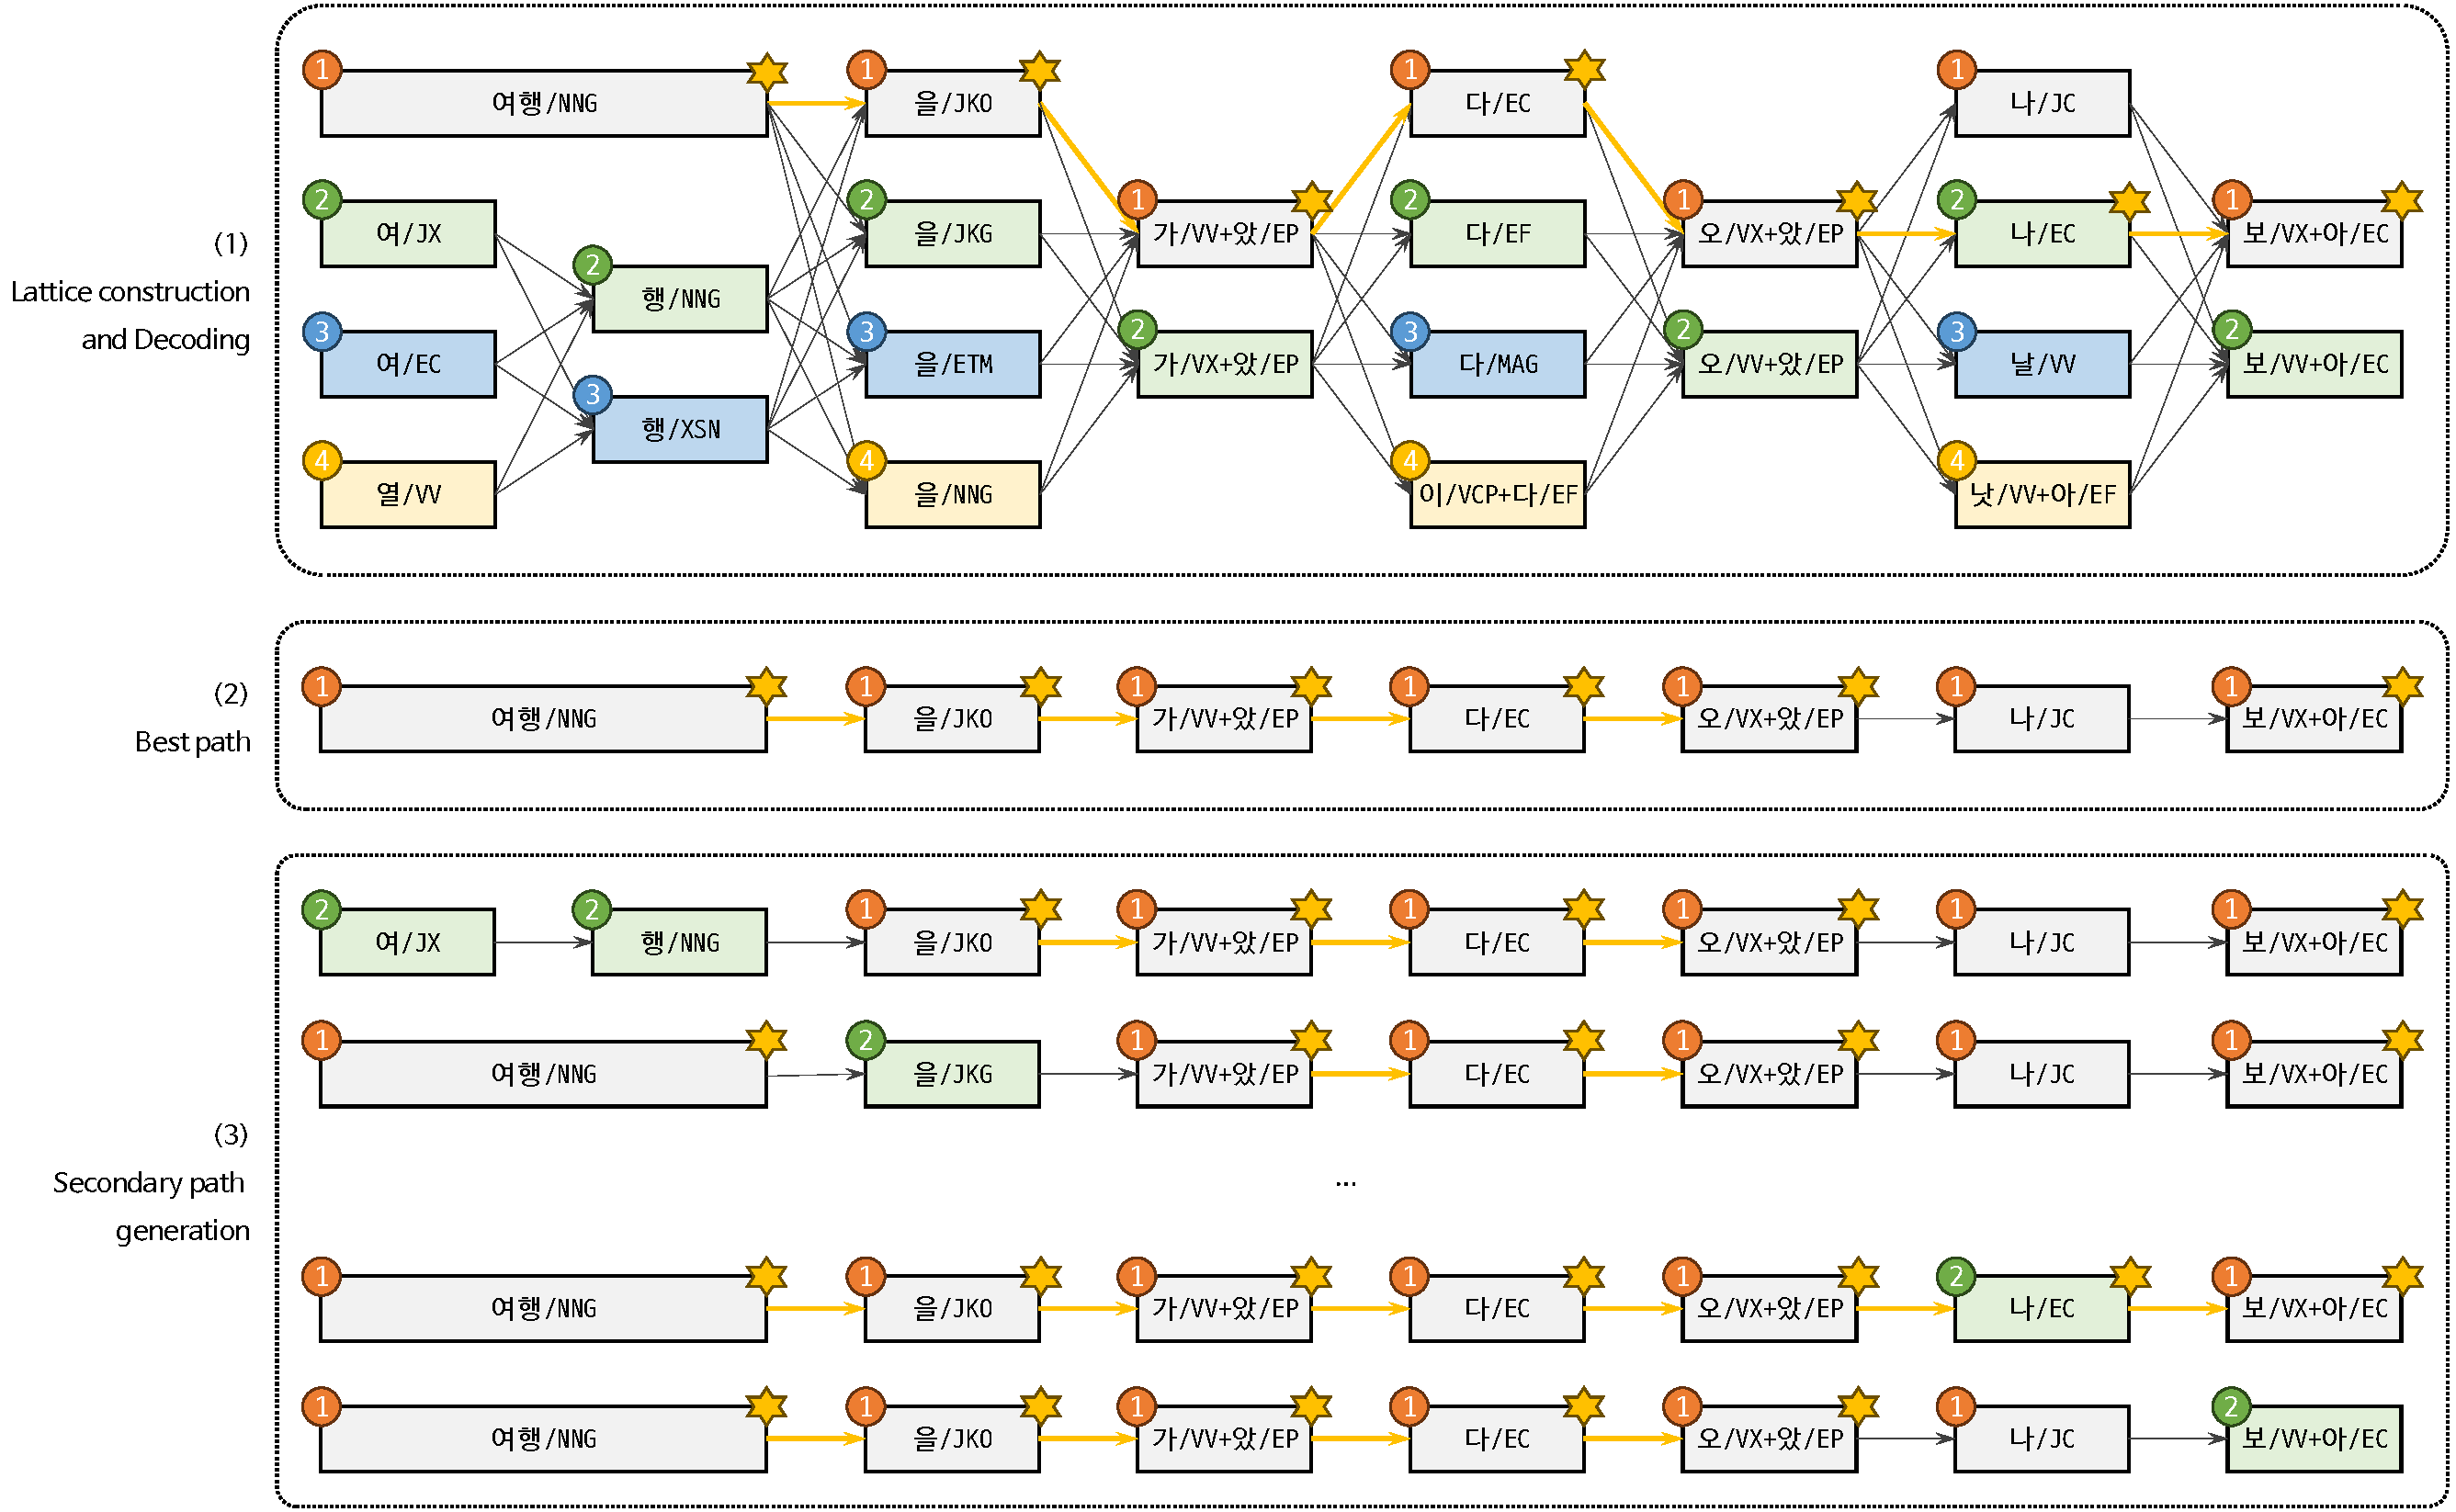
\includegraphics[width=0.9\textwidth]{fig2.1}}
        \caption{Example of lattice construction and decoding result and secondary path generation}\label{fig:lattice}
    \end{figure*}


    \section{Morphological Analysis Model}\label{sec:morphological-analysis-model}

    \subsection{Korean Morphological Analysis Corpora}\label{subsec3.1}

    A representative corpus for training Korean morphological analysis models is the Sejong morphological analysis corpus, which is often referred to as the Sejong corpus.
    The Sejong corpus, a major output of the 21st Century Sejong Project, contains 15 million words and is the mainstay of Korean morphological analysis research~\cite{ChoeMW2008}.

    Subsequent efforts have extended and refined this foundational work.
    The University of Ulsan addressed the limitations of the Sejong corpus~\cite{KimIH2010} and introduced [UCorpus], an expanded corpus of 63 million words.
    This expanded corpus not only adds new data but also corrects errors in the original Sejong corpus~\cite{UCorpusHG}.
    To further extend this step, the National Institute of Korean Language launched a massive Korean corpus construction project in 2018.
    The fruits of this labor, a corpus called <Everyone Corpus>, were released to the public in 2020~\cite{EveryoneCorpus}.
    A special offshoot of this project produced a morpheme-tagged corpus of three million words, including spoken languages ~\cite{KimIH2019}.

    \subsection{Training Example Transformation}\label{subsec3.2}

    To train a dictionary-based morpheme analysis model effectively, the morpheme-tagged corpus, typically represented in lemma form, must be transformed to include the boundary information between morphemes in its surface form.
    Crucial to this transformation is string alignment, a process that accounts for the discrepancies between lemma forms and surface forms in the Korean morphological analysis corpus.

    In this study, string alignment was performed using the Smith--Waterman algorithm, which uses a scoring matrix based on the similarity of the grapheme unit of Korean letters for each word pair (as shown in Figure~\ref{fig:sample}). Each aligned sentence containing a morpheme tag was converted into a training sample tailored for dictionary-based morphological analysis.

    The resulting table in Figure~\ref{fig:sample} illustrates this process.
    Each row acts as a lexical unit.
    The first four columns contribute to feature generation, whereas the last four columns facilitate post-lemmatization.
    Using the morphological corpus above, a large number of training samples can be generated according to the process shown in Figure~\ref{fig:sample}.
    With the exception of the evaluation samples, the remaining sentences were used to train the dictionary-based morphological analysis model using the CRF algorithm.
    The output of this training allowed the calculation of the costs associated with each morpheme node and the linking of two consecutive morphemes.
    This, in turn, allowed the discovery of an optimal path using the Viterbi algorithm.

    \begin{figure*}[t]
        \centerline{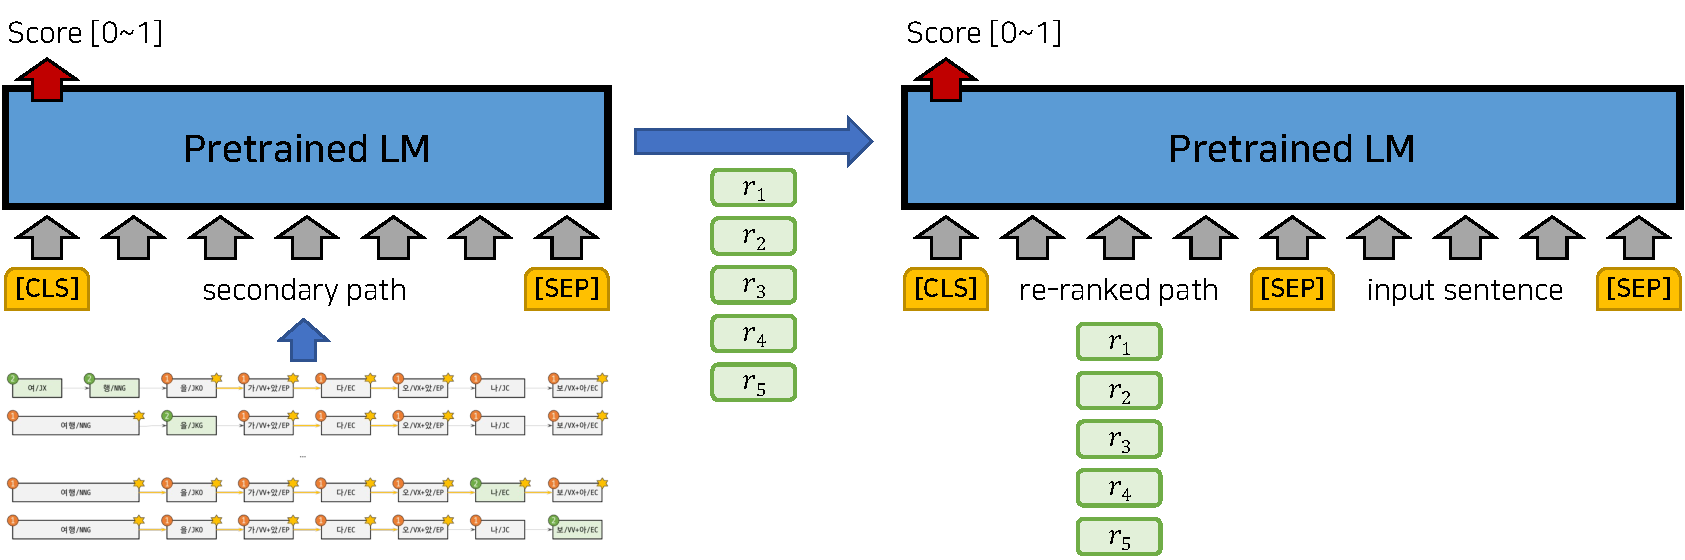
\includegraphics[width=0.9\textwidth]{fig3.0}}
        \caption{Two-stage re-ranking model for Korean morphological analysis}\label{fig:ranking}
    \end{figure*}

    \subsection{Lattice Construction and Decoding}\label{subsec3.3}

    Figure~\ref{fig:lattice} presents a snapshot of the lattice structure, which is an integral part of the morphological analysis.
    (1) shows a fragment of the lattice structure formed when the example sentence in Figure~\ref{fig:sample} is entered.
    (2) shows the optimal path determined using the Viterbi algorithm.

    However, the path inferred by the trained model may differ from the correct solution constructed by humans.
    The nodes marked with stars in (1) represent correct nodes.
    The upper-left number of each node indicates the ranking of the nodes accessible at each decoding point.
    The choices made at certain moments deviate from the correct solution.
    To improve analytical performance, mechanisms to correct these discrepancies must developed.


    \section{Re-ranking Model}\label{sec:re-ranking-model}

    \subsection{Motivation and Background}\label{subsec4.1}

    Although dictionary-based morphological analysis offers significant advances, its optimal paths occasionally diverge from the correct solutions that humans understand.
    This divergence underscores the need for a model that reevaluates these primary results and reorients them to achieve higher accuracy.
    This method, called "re-ranking," involves generating multiple analyses of an input and then reordering them based on a new set of criteria or models, thereby improving the overall quality of the results.

    \subsection{Secondary Path Generation}\label{subsec4.2}

    Before reranking begins, multiple analyses, typically referred to as the N-best paths, of the input sentence are generated.
    This involves extracting the top N atoms from the lattice structure.
    In this study, a novel approach is introduced to generate secondary paths, as shown in (3) of Figure~\ref{fig:lattice}, by selecting the second-best node rather than each best node constituting the path from the best-path result.
    Some of these secondary paths provided alternatives that reconciled incorrect with correct answers.
    Similarly, paths modified by favoring the third-best node were called tertiary paths, and this naming convention was continued for subsequent paths.
    In our preliminary test, the secondary paths, including the optimal and suboptimal paths, were shown to cover the majority of the correct morphological analyses as measured through human evaluations. (Refer to Table~\ref{tab:maximum-performance}).

    \subsection{BERT-based Re-ranking}\label{subsec4.3}

    Bidirectional Encoder Representations from Transformers (BERT) models~\cite{Devlin2019} have revolutionized many natural language processing tasks by understanding the context in which words appear in text.
    In this study, we attempt to leverage the power of BERT to reorder the generated secondary paths.
    We labeled the generated secondary paths with scores related to the morphological analysis performance to fine-tune a pre-trained BERT model specialized for Koreans with excess amount Korean text.
    After pre-testing several scoring methods on a modest scale, we found that using scores based on the degree of error rather than scores based on accuracy by widen the gap between correct and incorrect answers is effective for learning.

    Once the BERT model is fine-tuned and trained for the re-ranking task, it can predict a re-ranking score for each path in the secondary path list.
    This implies that considering the context, morphological organization, and other essential linguistic features of the path, the model assigns a score to each path.
    The paths were then re-ranked according to this score, and the path with the highest score was selected for the best morphological analysis.

    \begin{table*}[]
        \caption{Statistics on full data for training and evaluating three morphological analysis models}\label{tab:data-statistics}
        \centering
        \begin{tabular*}{500pt}{@{\extracolsep\fill}|c|c|rrr|rrr|@{\extracolsep\fill}}
            \toprule
            \multicolumn{2}{|c|}{\multirow{2}{*}{\textbf{Corpus}}} & \multicolumn{3}{c|}{\textbf{Training Set}} & \multicolumn{3}{c|}{\textbf{Test Set}} \\
            \cmidrule{3-5} \cmidrule{6-8}
            \multicolumn{2}{|c|}{~} & sentences & eojeols & morphemes & sentences & eojeols & morphemes \\
            \midrule
            \multicolumn{2}{|c|}{Sejong Corpus} & 194,822 & 2,681,582 & 6,033,785 & 49,922 & 678,578 & 1,527,803 \\
            \midrule
            \multirow{3}{*}{UCorpus}         & written     & 4,998,560 & 57,393,332 & 127,171,473 & 53,003 & 598,413 & 1,325,419 \\
            ~                                & semi-spoken & 334,061   & 2,960,146  & 6,468,494   & 38,960 & 332,285 & 726,398   \\
            ~                                & spoken      & 429,215   & 2,295,940  & 5,584,494   & 62,399 & 279,545 & 691,542   \\
            \midrule
            \multirow{2}{*}{Everyone Corpus} & written     & 129,352   & 1,713,367  & 3,944,118   & 14,442 & 191,223 & 440,052   \\
            ~                                & spoken      & 137,869   & 714,021    & 1,440,746   & 19,789 & 85,316  & 170,523   \\
            \bottomrule
        \end{tabular*}
    \end{table*}

    \subsection{Two-stage Re-ranking}\label{subsec4.4}

    Given the complexity of the Korean language, a single re-ranking step does not constantly yield accurate results.
    Therefore, we propose a two-step re-ranking approach as described in ~\cite{Nogueira2019}.

    In the first step, we re-rank the secondary paths generated using the BERT model, as described in Section ~\ref{subsec4.3}.
    In the second step, we introduced another BERT variant that was optimized for a different set of linguistic features or trained on a different dataset.
    This allowed us to perform a fine-grained re-evaluation, further refine the list, and push more contextually accurate paths to the top.

    As shown in Figure~\ref{fig:ranking}, for a two-stage reranking model, the first stage performs the first re-ranking, taking as input a secondary path in morphologically tagged lemma form.
    It then performs a second re-ranking, again taking as input the path re-ranked in stage 1 and the original input sentence.
    This was conducted to improve effectiveness, as it was ineffective given the same type of input.


    \section{Experimental Results}\label{sec:results}

    We evaluated the performance of the proposed deep learning-integrated dictionary-based morphological analysis method.
    This section presents the results of the experimental evaluation considering the improvements over conventional methods and the effectiveness of our re-ranking model.

    \subsection{Setup and Data}\label{subsec5.1}

    For our experiments, we used the Sejong corpus (versions used in ~\cite{NaSH2014, NaSH2015, NaSH2018, SongHJ2019, SongHJ2020}), UCorpus\cite{UCorpusHG}, and Everyone Corpus\cite{EveryoneCorpus}.
    For comparison with previous studies, the Sejong corpus was trained using a single model without separation.
    The UCorpus and Everyone Corpus provided a separate spoken corpus with drama scripts and broadcast dialogues, while UCorpus separated documents that were considered to be close to spoken language and further organized them into a semi-spoken corpus.
    Because UCorpus and Everyone Corpus have synergistic effects when trained concurrently, we trained the models separately for written and spoken language rather than separating them by source.
    The statistics of the full data for the three types of models are presented in Table~\ref{tab:data-statistics}.
    Because of the large volume of UCorpus, we randomly selected some of them to train the actual model.

    We transformed this organized morphological corpus using the training-example transformation process described in Section ~\ref{subsec3.2} to generate samples for training the dictionary-based morphological analysis model.

    \begin{table*}[]
        \caption{Performance comparison between morphological analysis systems without re-ranking}\label{tab:performance-without-reranking}
        \begin{tabular*}{500pt}{@{\extracolsep\fill}c|cccccc@{\extracolsep\fill}}
            \toprule
            \multirow{2}{*}{System} & \multicolumn{2}{c}{Sejong} & \multicolumn{2}{c}{UCorpus (written)} & \multicolumn{2}{c}{Everyone Corpus (written)} \\
            \cmidrule{2-3} \cmidrule{4-5} \cmidrule{6-7}
            & \multicolumn{1}{c}{eojeol} & \multicolumn{1}{c}{morpheme} & \multicolumn{1}{c}{eojeol} & \multicolumn{1}{c}{morpheme} & \multicolumn{1}{c}{eojeol} & \multicolumn{1}{c}{morpheme} \\
            \midrule
            \hspace{2mm}MeCab-ko                   & 89.17                      & 93.06                        & 87.88                      & 92.32                        & 87.77                      & 92.05                        \\
            \hspace{2mm}Syllable-based (written)   & 91.95                      & 95.16                        & \textbf{96.84}             & \textbf{97.97}               & \textbf{98.00}             & \textbf{98.82}               \\
            \hspace{2mm}Dictionary-based (written) & 90.99                      & 94.58                        & 96.33                      & 97.74                        & 96.85                      & 98.14                        \\
            \hspace{2mm}Dictionary-based (Sejong)  & \textbf{95.23}             & \textbf{97.08}               & 90.18                      & 94.19                        & 91.30                      & 94.79                        \\
            \toprule
            \multirow{2}{*}{System} & \multicolumn{2}{c}{UCorpus (semi-spoken)} & \multicolumn{2}{c}{UCorpus (spoken)} & \multicolumn{2}{c}{Everyone Corpus (spoken)} \\
            \cmidrule{2-3} \cmidrule{4-5} \cmidrule{6-7}
            & \multicolumn{1}{c}{eojeol} & \multicolumn{1}{c}{morpheme} & \multicolumn{1}{c}{eojeol} & \multicolumn{1}{c}{morpheme} & \multicolumn{1}{c}{eojeol} & \multicolumn{1}{c}{morpheme} \\
            \midrule
            \hspace{2mm}MeCab-ko                   & 86.85                      & 91.38                        & 81.75                      & 87.90                        & 85.28                      & 89.52                        \\
            \hspace{2mm}Syllable-based (spoken)    & \textbf{96.56}             & \textbf{97.65}               & \textbf{94.89}             & \textbf{96.76}               & \textbf{95.14}             & \textbf{96.82}               \\
            \hspace{2mm}Dictionary-based (spoken)  & 94.98                      & 96.65                        & 93.02                      & 95.71                        & 92.47                      & 94.83                        \\
            \bottomrule
        \end{tabular*}
    \end{table*}

    \subsection{Evaluation Metrics}\label{subsec5.2}

    To measure the accuracy of the morphological analysis model, correctness of the N-best path, and ranking accuracy of the reranking model, we used the eojeol accuracy and morpheme F1 scores as evaluation metrics.
    To verify that they produced the correct morphological analysis results, we measured the degree of agreement with human annotations on the corpus.
    However, owing to the slightly different criteria and styles of the annotators who labeled the different types of corpora, including the comparison with the MeCab-ko system, the following adjustments were made:
    \begin{itemize}
        \item Sentences containing unanalyzable tags (NF, NA, and NV) were excluded from both training and evaluation.
        \item As for the tagsets, we excluded three unanalyzable tags from the 45 Sejong tagsets and used 42 tagsets.
        \item Each tag output by the MeCab-ko system was converted to the corresponding tag in the Sejong tagset.
        \item Chinese characters were converted to Chinese character tags (SH) even if they were semantically used as nouns, and consecutive Chinese characters were converted to a single morpheme.
        \item Similarly, symbol, numeral, ending, and postposition in the same tag were converted to a single morpheme, and decimal expressions were treated as a single morpheme, including the midpoint and the numbers before and after.
        \item If the first lemma letter of the ending is `[eo]', `[yeo]', or `[ah]', it is unified as `[eo]', and if it is `[eot]', `[yeot]', or `[ass]', it is unified as `[eot]'. %`어[eo]', `여[yeo]', or `아[ah]' % `었[eot]', `였[yeot]', or `았[ass]'
        \item Root tags (XR) used alone without affixes were replaced with common nouns (NNG) because they are mainly used in the Sejong corpus only.
        \item As mentioned in ~\cite{KimIH2010}, connective endings (EC) and sentence-closing endings (EF) are not clearly defined in the tagging guidelines, and there are cases where they are used interchangeably in the corpus, to ensure that we evaluated them without distinguishing them.
        \item The distinction between `[geot]' and `[geo]' is unclear in the tagging guidelines, and there are cases where they are used interchangeably in the corpus, hence, we did not distinguish between them. %`것[geot]' and `거[geo]'
        \item Compound words can be interpreted as a single morpheme or as a combination of two or more morphemes or affixes, hence, we evaluated them without distinguishing between them.
        \item Proper nouns can also be interpreted as common nouns depending on the point of view or perspective. Human annotators have slightly different standards, and thus they were also evaluated without distinguishing the nouns.
    \end{itemize}

    \subsection{Basic Performance}\label{subsec5.3}

    First, we compared the initial results of the dictionary-based morphological analysis model trained using the method described in Section ~\ref{sec:morphological-analysis-model} with those of MeCab and syllable-based morphological analysis systems (refer to Table~\ref{tab:performance-without-reranking}).
    The results show that the dictionary-based method implemented is superior to the existing MeCab system, but it differs from human evaluations owing to the limitations mentioned above, and it does not reach the performance of existing syllable-based morphological analysis systems.
    We also found that the compatibility between the Sejong corpus and other corpora is poor, as the model trained on the Sejong corpus has guaranteed performance when evaluated on the Sejong corpus, and some performance degradation occurs on other corpora.

    \begin{table*}[]
        \caption{Performance comparison between morphological analysis systems with Two-stage re-ranking}\label{tab:performance-with-reranking}
        \begin{tabular*}{500pt}{@{\extracolsep\fill}c|cccccc@{\extracolsep\fill}}
            \toprule
            \multirow{2}{*}{System} & \multicolumn{2}{c}{Sejong} & \multicolumn{2}{c}{UC+EC (written)} & \multicolumn{2}{c}{UC+EC (spoken)} \\
            \cmidrule{2-3} \cmidrule{4-5} \cmidrule{6-7}
            & \multicolumn{1}{c}{eojeol} & \multicolumn{1}{c}{morpheme} & \multicolumn{1}{c}{eojeol} & \multicolumn{1}{c}{morpheme} & \multicolumn{1}{c}{eojeol} & \multicolumn{1}{c}{morpheme} \\
            \midrule
            \hspace{2mm}MeCab-ko                          & 89.17                      & 93.06                        & 87.83                      & 92.19                        & 84.62                      & 89.60                        \\
            \hspace{2mm}Syllable-based                    & 91.95                      & 95.16                        & 97.42                      & 98.39                        & 95.53                      & \textbf{97.08}               \\
            \hspace{2mm}Dictionary-based (without rerank) & 95.23                      & 97.08                        & 96.59                      & 97.94                        & 93.49                      & 95.73                        \\
            \hspace{2mm}Dictionary-based (1-stage rerank) & 96.63                      & 97.84                        & 97.50                      & 98.44                        & 94.77                      & 96.62                        \\
            \hspace{2mm}Dictionary-based (2-stage rerank) & \textbf{96.87}             & \textbf{98.01}               & \textbf{97.75}             & \textbf{98.60}               & \textbf{95.56}             & \textbf{97.08}               \\
            \bottomrule
        \end{tabular*}
    \end{table*}

    \subsection{Re-ranking Performance}\label{subsec5.4}

    Upon integrating the BERT-based re-ranking model, we observed substantial performance enhancement.
    Table~\ref{tab:performance-with-reranking} shows that the re-ranking model identified a better path in a significant proportion of cases.
    The first-stage re-ranking exhibited a performance improvement of over 20\% compared with traditional models.
    The subsequent re-ranking, leveraging a distinct type of input and a different pre-trained model, further augmented the performance by more than 30\%.

    Next, we performed the BERT-based re-ranking described in Section ~\ref{sec:re-ranking-model} and compared its performances.
    Three pre-trained language models, KPF-BERT, ETRI-ELECTRA, and ETRI-RoBERTa, which are known to perform well in other Korean language understanding tasks, were used to fine-tune the re-ranking model.
    KPF-BERT received Korean sentences as input, ETRI-ELECTRA received morphologically tagged sentences as input, and ETRI-RoBERTa receives morpheme-separated sentences as input.
    For KPF-BERT and ETRI-RoBERTa, there may be problems with model learning because of the separation of morpheme tags into letter units during the tokenization process when the morpheme analysis results were received as input and re-ranked, hence, the morpheme tags of the mid-level classification unit were added as new tokens, and then training was performed.
    As shown in Figure~\ref{fig:ranking}, for these three types of pre-trained language models, we first performed training with a re-ranking model using only the morphological analysis results and then performed training with a second re-ranking model using the top five morphological analysis results from the first re-ranking results along with the input sentences for other types of pre-trained language models.
    Preliminary tests indicate that using the same type of model or input results in a nearly identical retrained model, with no further improvement in performance.

    The sentences used for training the re-ranking model were selected from those used for training the dictionary-based morphological analysis model: 190,000 sentences from the Sejong corpus, 240,000 sentences from the written language of the combined UCorpus and Everyone corpus, and 360,000 sentences from the spoken language of the combined UCorpus and Everyone corpus.
    For a large number of sentences, we adopted a floating-point 16-bit technique while using four GPUs for distributed training and significantly reduced the time required for training.
    In addition, the minibatch size was 120 with a maximum sequence length of 384 because the first re-ranking uses only the morphological analysis results as input.
    The minibatch size was 40 with a maximum sequence length of 512 because the original input sentences were given as input along with the first morphological analysis results.
    The learning rate was set to $2 \times 10^{-5}$ and AdamW is used as the optimization algorithm.

    Table~\ref{tab:performance-with-reranking} shows that incorporating the re-ranking model significantly improves the performance compared with no re-ranking.
    The error reduction rate (ERR) of the performance change from the existing model on eojeol accuracy is shown as 29\%, 27\%, and 20\% for the Sejong corpus, combined written corpus, and combined spoken corpus, respectively, with the first round of re-ranking, and the second round of re-ranking improved the performance by increasing the rate to 34\%, 34\%, and 32\%, respectively.
    These performance improvements demonstrate that the dictionary-based morphological analysis model outperforms traditional syllable-based morphological analysis systems, including numerous pre- and post-processing rules and dictionaries.

    \begin{table*}[]
        \caption{Comparison of performance differences with previous studies}\label{tab:differences-with-previous-studies}
        \begin{tabular*}{500pt}{@{\extracolsep\fill}ccc|cc@{\extracolsep\fill}}
            \toprule
            \multirow{2}{*}{Authors} & \multirow{2}{*}{Model} & \multirow{2}{*}{Data (train, test)} & \multicolumn{2}{c}{Performance} \\
            \cmidrule{4-5}
            ~                                     & ~                                          & ~                                           & \multicolumn{1}{c}{eojeol} & \multicolumn{1}{c}{morpheme} \\
            \midrule
            Na, 2015~\cite{NaSH2015}              & CRF++, HMM                                 & Sejong 200k, 50k sentences                  & 95.22                      & 97.21                        \\
            Lee et al., 2016~\cite{LeeCH2016}     & Structural SVM                             & Sejong 666k, 74k eojeols                    & 96.41                      & -                            \\
            Li et al., 2017~\cite{Li2017}         & Seq2seq (GRU-based)                        & Sejong 90k, 10k sentences                   & 95.33                      & 97.15                        \\
            Na and Kim, 2018~\cite{NaSH2018}      & Lattice + HMM                              & Sejong 200k, 50k sentences                  & 96.35                      & 97.74                        \\
            Min et al., 2019~\cite{MinJW2019}     & Seq2seq (Transition-based)                 & Sejong 200k, 50k sentences                  & 96.34                      & 97.68                        \\
            Song and Park, 2019~\cite{SongHJ2019} & Seq2seq (BiLSTM-based)                     & Sejong 200k, 50k sentences                  & 95.68                      & 97.43                        \\
            Youn et al, 2021~\cite{YounJY2021}    & Seq2seq (BERT-based)                       & Sejong 675k, 75k sentences                  & 95.99                      & 97.94                        \\
            Shin et al, 2023~\cite{ShinHJ2023}    & Transformer(En) + BiLSTM                   & Sejong 769k, 87k sentences                  & 96.12                      & 97.74                        \\
            \midrule
            Proposed (without rerank)             & \multirow{3}{*}{Lattice + Transformer(En)} & \multirow{3}{*}{Sejong 194k, 10k sentences} & 95.23                      & 97.08                        \\
            Proposed (1-stage rerank)             & ~                                          & ~                                           & 96.63                      & 97.84                        \\
            Proposed (2-stage rerank)             & ~                                          & ~                                           & \textbf{96.87}             & \textbf{98.01}               \\
            \bottomrule
        \end{tabular*}
    \end{table*}

    \subsection{Comparison to Other Studies}\label{subsec5.5}

    We found that the proposed transformer-based re-ranking technique consistently improved the results of the existing morphological analysis models.
    These results open new possibilities in the area of Korean morphological analysis by further improving the results of existing traditional machine learning models.
    Finally, because the results of the major related works proposed in the literature were mostly conducted on the Sejong corpus, we compared the performance improvement of the Sejong corpus with the results of previous studies.

    We found that the proposed transformer-based re-ranking technique consistently improved the results of the existing morphological analysis models.
    These results confirm that it opens up new possibilities by further improving the results of existing traditional machine-learning models in the field of Korean morphological analysis.
    Finally, because the major related studies proposed in the literature were mostly conducted on the Sejong corpus, we compared the performance improvement of the Sejong corpus with the results of previous studies.
    Although it is difficult to make a direct comparison because of slight differences in implementation conditions and evaluation criteria.
    The proposed dictionary-based morphological analysis model is not up to the latest research results; however, by incorporating a re-ranking model, it can secure a performance that is comparable to existing research.

    The entire morphological analysis model, including the re-ranking model, is not suitable for real-time processing.
    However, it is expected that by reflecting the cases whose ranks are changed through the re-ranking model as feedback to the dictionary-based morphological analysis model, it will be feasible to obtain near-improved morphological analysis performance.
    The improved dictionary-based morphological analysis model can then be used as input to the re-ranking model; therefore, it is expected that a gradually improvement in morphological analysis model can be obtained through this iterative feedback loop.


    \section{Conclusion}\label{sec:conclusion}

    This study signifies a progressive stride in Korean morphological analysis by seamlessly merging conventional dictionary-based techniques with advanced deep learning methodologies.
    Our findings indicate that while relying solely on dictionary-based morphological analysis does not surpass the efficacy of some existing models, the integration of a BERT-based re-ranking system notably enhances accuracy, establishing a new standard in this domain.

    While the performance improvement increases computational demand, the introduced methodology provides a promising avenue for continuous enhancement.
    This innovative amalgamation of classical dictionary approaches and cutting-edge machine-learning methodologies paves the way for groundbreaking advancements in the intricate and multifaceted domains of Korean linguistic processing.

    Future endeavors in this domain should emphasize the refinement of this harmonious integration to achieve even higher precision in morphological analysis while optimizing computational efficiency.
    Moreover, our observations indicate the potential for employing a probabilistic model to discern areas where inaccuracies are likely to arise, thus enabling the retrieval of more accurate interpretations from a narrower candidate pool.
    The parallels between this initiative and the challenges of translation quality estimation suggest that insights from the latter can bolster the efficacy of our approach.


    \bibliography{references}

\end{document}
